Que faire si nous avons des formules trigonométriques impliquant deux variables, ou plus?
Par exemple,
pour
$(\alpha ; \beta) \in \big( \RRsp \big)^2$ tel que $0 < \alpha + \beta < \frac{\pi}{2}$,
le dessin suivant nous donne
$\cos(\alpha + \beta) = \cos \alpha \cos \beta - \sin \alpha \sin \beta$
et
$\sin(\alpha + \beta) = \cos \alpha \sin \beta + \sin \alpha \cos \beta$.%
\footnote{
    Cette démonstration est très utile pour un cours pré universitaire.
}
Nous allons voir comment passer à $(\alpha ; \beta) \in \CC^2$.


\begin{center}
	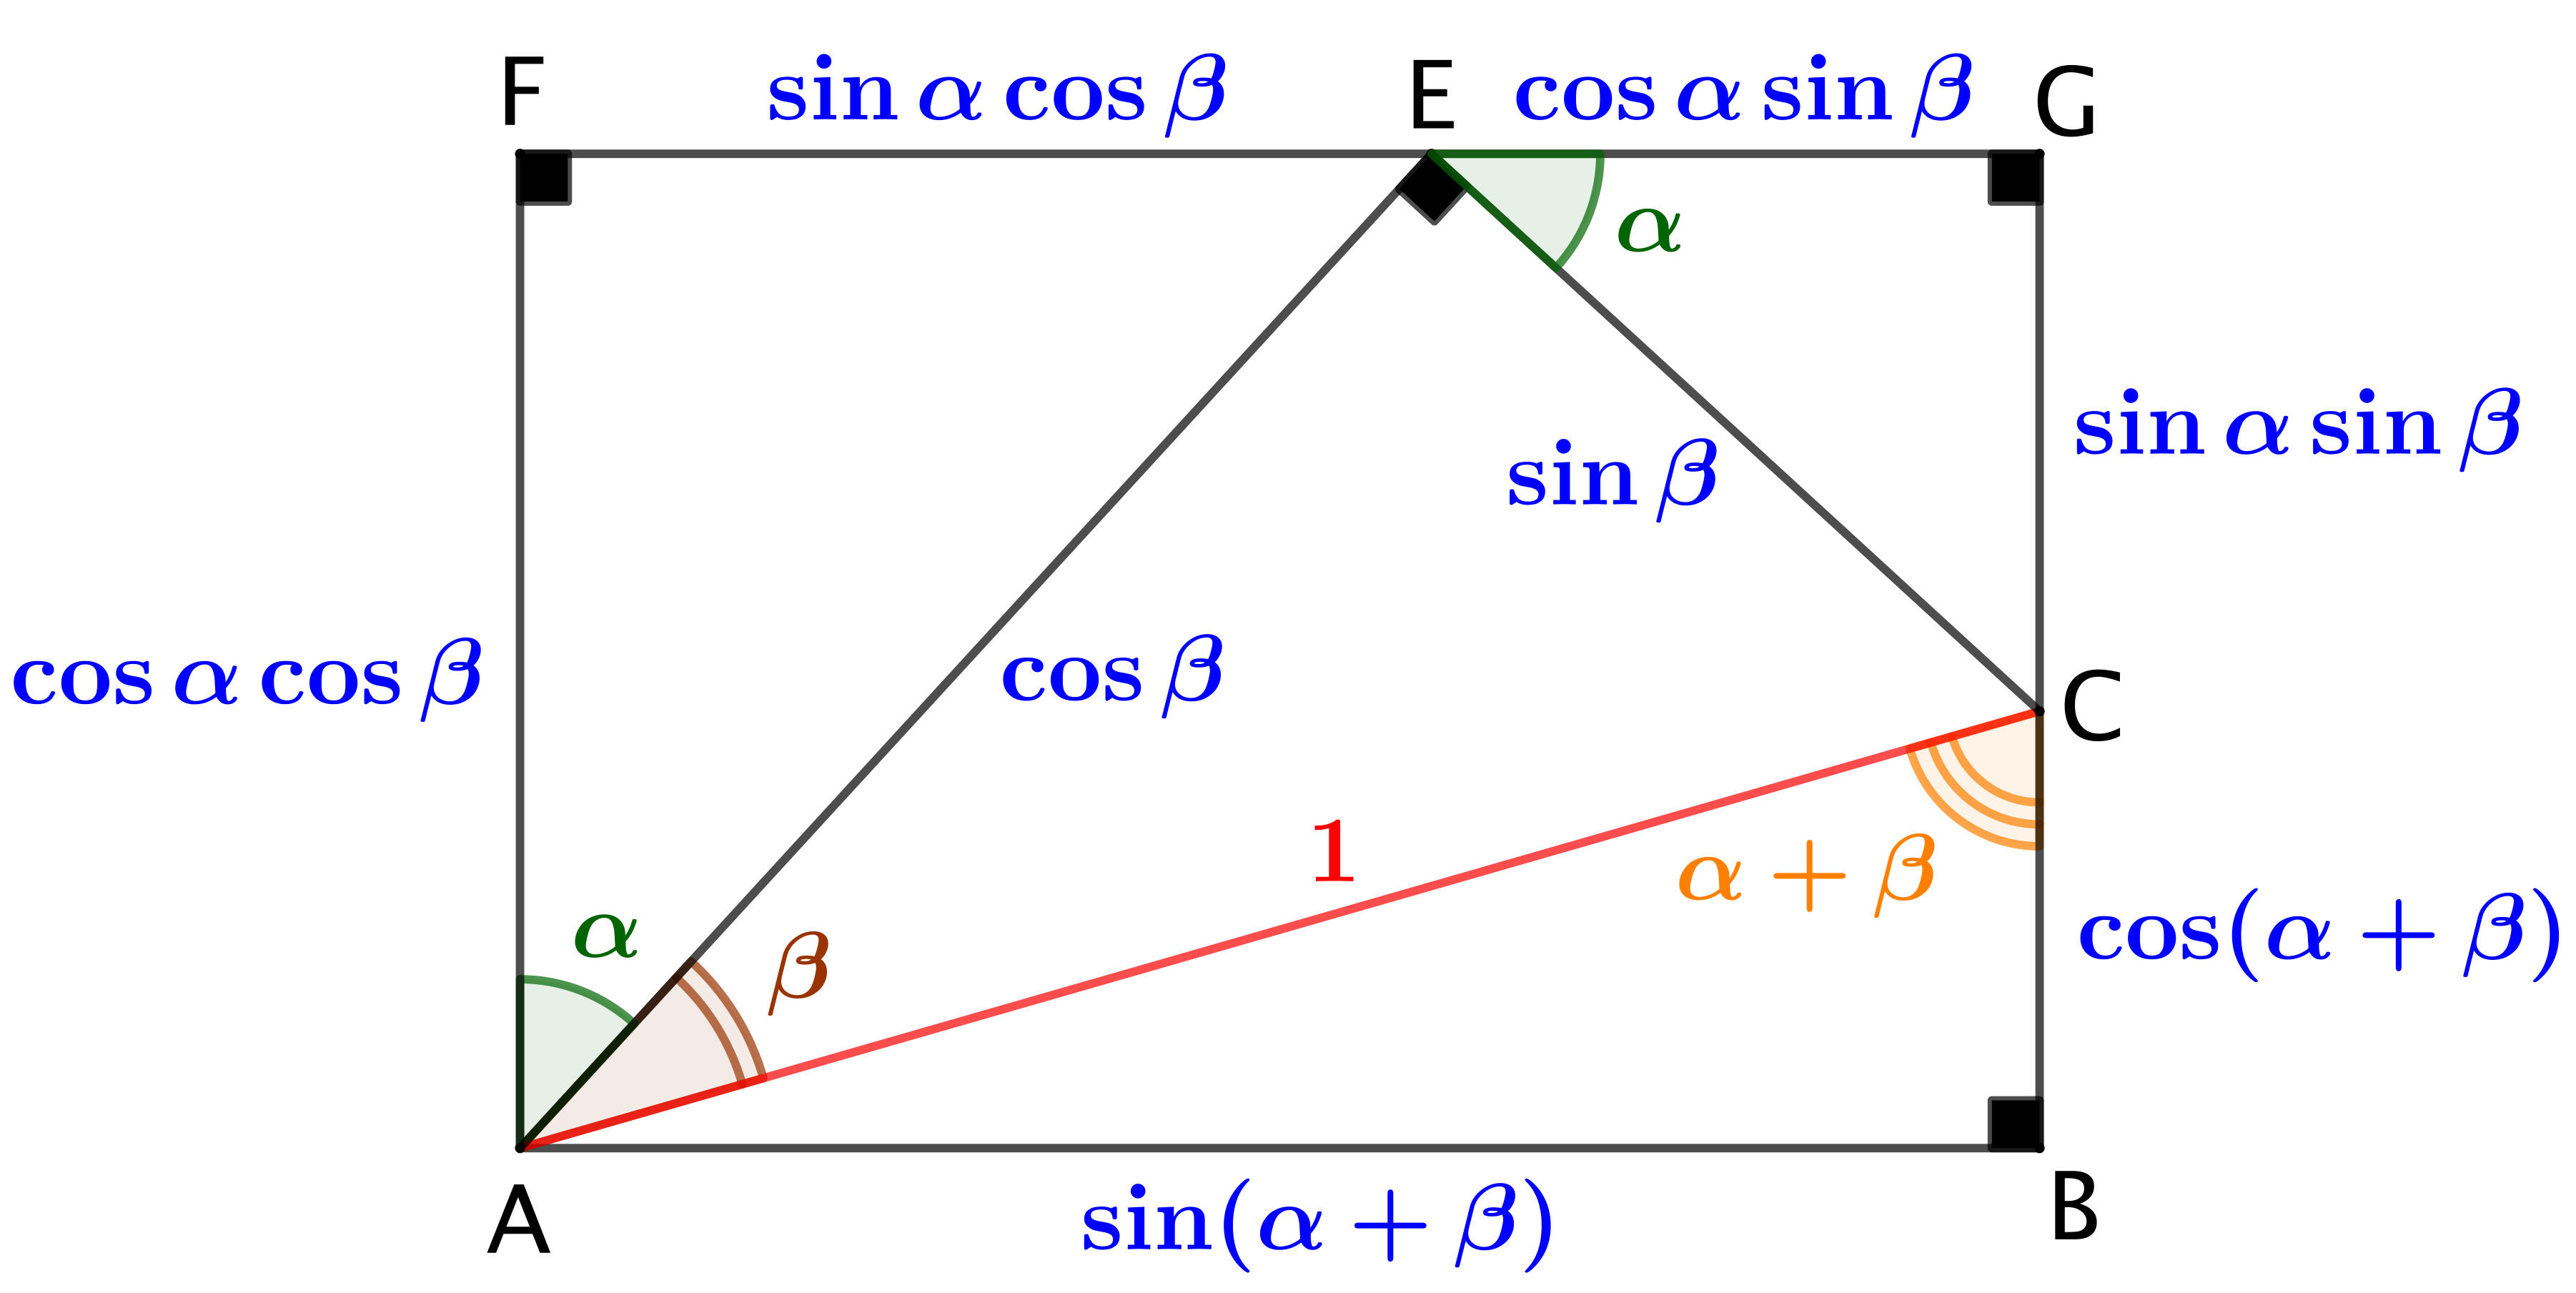
\includegraphics[scale=.7]{add-trigo-formulas.png}
\end{center}


% ----------- %


\begin{defi}
    Soit $n \in \NNs$.
    %
    Pour toute fonction $f: \CC^n \rightarrow \CC$
    et
    $k \in \ZintervalC{1}{n}$,
    nous nommerons \focus{k\ieme\ restriction de $f$} relativement à $(z_1 ; ... ; z_{k-1} ; z_{k+1} ; ... ; z_n) \in \CC^{n-1}$ 
    la fonction $f_{k , z_{\small\bullet}}$ définie sur $\CC$ par
    $f_{k , z_{\small\bullet}}(z) = f(z_1 ; ... ; z_{k-1} ; z ; z_{k+1} ; ... ; z_n)$.
\end{defi}


\begin{defi}
    Soit $n \in \NNs$.
    %
    Une fonction $f: \CC^n \rightarrow \CC$ sera dite \focus{séparablement analytique} sur $\CC^n$,
    si $\forall k \in \ZintervalC{1}{n}$,
    toutes ses k\iemes\ restrictions $f_{k , z_{\small\bullet}}$ sont analytiques.
\end{defi}


\begin{defi}
    L'ensemble $\setgeo{E} \subseteq \CC$ sera dit \focus{discriminant} 
    s'il existe $\omega \in \setgeo{E}$ non isolé,
    c'est-à-dire
    que pour tout réel $r > 0$,
    $\CdiscO{\omega}{r} \cap \setgeo{E}$ possède au moins deux éléments.
    %
    Plus généralement,
    si $\prod_{k=1}^{n} \setgeo*{E}{k}$ où chaque $\setgeo*{E}{k} \subseteq \CC$ est discriminant,
    nous dirons que
    $\prod_{k=1}^{n} \setgeo*{E}{k}$ est discriminant.
\end{defi}


\begin{fact} \label{sep-isolated-zero}
    Soient $n \in \NNs$
    et
    $f: \CC^n \rightarrow \CC$ une fonction séparablement analytique.
	Si $f$ s'annule sur $\prod_{k=1}^{n} \setgeo*{E}{k}$ discriminant,
	alors $f$ s'annule sur $\CC^n$ tout entier. 
\end{fact}


\begin{proof}
	Comme le schéma de démonstration est similaire à celui de la preuve du \reffact{poly-nullity-pos},
	nous donnons juste les grandes étapes permettant de raisonner par récurrence sur $n \in \NNs$.
	Pour cela, considérons $\setproba{P}(n)$ définie par
	\emph{\og 
		Pour toute fonction séparablement analytique $f: \CC^n \rightarrow \CC$,
		si $f$ s'annule sur $\prod_{k=1}^{n} \setgeo*{E}{k}$ où chaque $\setgeo*{E}{k} \subseteq \CC$ est discriminant,
		alors $f$ s'annule sur $\CC^n$. 
	\fg}\kern2pt.
	%
	\begin{itemize}[label=\small\textbullet]
		\item \textbf{Cas de base.}
		%
		$\setproba{P}(1)$ découle directement du \reffact{isolated-zero}.


		\item \textbf{Hérédité.}
		%
		Soit $f$ une fonction séparablement analytique à $(n + 1)$ variables vérifiant les conditions de la propriété $\setproba{P}(n + 1)$
		avec
		$\prod_{k=1}^{n+1} \setgeo*{E}{k}$ l'ensemble sur lequel $f$ est nulle.
		%
		Pour $\omega \in \setgeo*{E}{n+1}$,
		en posant
		$f_\omega: (z_1 ; ... ; z_n) \in \CC^n \mapsto f(z_1 ; ... ; z_n ; \omega) \in \CC$,
		nous avons $f_\omega$ validant $\setproba{P}(n)$.
		%
		Donc, $\forall (z_1 ; ... ; z_n) \in \CC^n$,
		posant $\ell(z) = f(z_1 ; ... ; z_n ; z)$,
		nous obtenons $\ell$ vérifiant $\setproba{P}(1)$.
		%
		Finalement,
		$f(z_1 ; ... ; z_n ; z)$ est nulle sur $\CC^{n+1}$.
	\end{itemize}

	\null\vspace{-6ex}
\end{proof}


% ----------- %


%\newpage
\begin{example}
    Le \reffact{sep-isolated-zero} implique la validité des formules trigonométriques d'addition sur $\CC^2$ tout entier en considérant les fonctions
    $f_1(\alpha ; \beta) = \cos(\alpha + \beta) - \cos \alpha \cos \beta + \sin \alpha \sin \beta$
    et
    $f_2(\alpha ; \beta) = \sin(\alpha + \beta) - \cos \alpha \sin \beta - \sin \alpha \cos \beta$
    qui s'annulent sur $\intervalO{0}{\frac{\pi}{4}}^2$.
\end{example}


% ----------- %


%\newpage
\begin{example}
    L'implication
    $\big[
        \alpha + \beta + \gamma = \frac{\pi}{2}
        \implies
          \tan \alpha \tan \beta
        + \tan \beta  \tan \gamma
        + \tan \gamma \tan \alpha
        = 1
    \big]$
    est vraie pour 
    $(\alpha ; \beta ; \gamma) \in \intervalO{0}{\frac{\pi}{2}}^3$,
    comme le montre le dessin suivant.
    Il est naturel de se demander s'il est possible de partir, plus généralement, de
    $(\alpha ; \beta ; \gamma) \in \big( \CC - \frac{\pi}{2} \ZZ \big)^3$.
    Nous allons voir que c'est bien le cas.
    %
    \footnote{
    	Ici, il est aisé de faire une vérification directe, mais cela sort de l'esprit de ce document, et est non généralisable.
		%
		En effet,
		en multipliant l'égalité souhaitée par $\cos \alpha \cos \beta \cos \gamma$, nous devons démontrer que
		$ \sin \alpha \sin \beta \cos \gamma
        + \cos \alpha \sin \beta \sin \gamma
        + \sin \alpha \cos \beta \sin \gamma
        - \cos \alpha \cos \beta \cos \gamma
        = 0$.
        Dans le terme de gauche, les formules d'addition se cachent de façon ostentatoire.
        Nous obtenons
		$ \sin \alpha \sin(\beta + \gamma)
        - \cos \alpha \cos(\beta + \gamma)$,
        puis
		$ - \cos (\alpha + \beta + \gamma)$,
        soit
		$- \cos (\frac{\pi}{2})$
		qui est bien nul.
    }
    
    \begin{center}
    	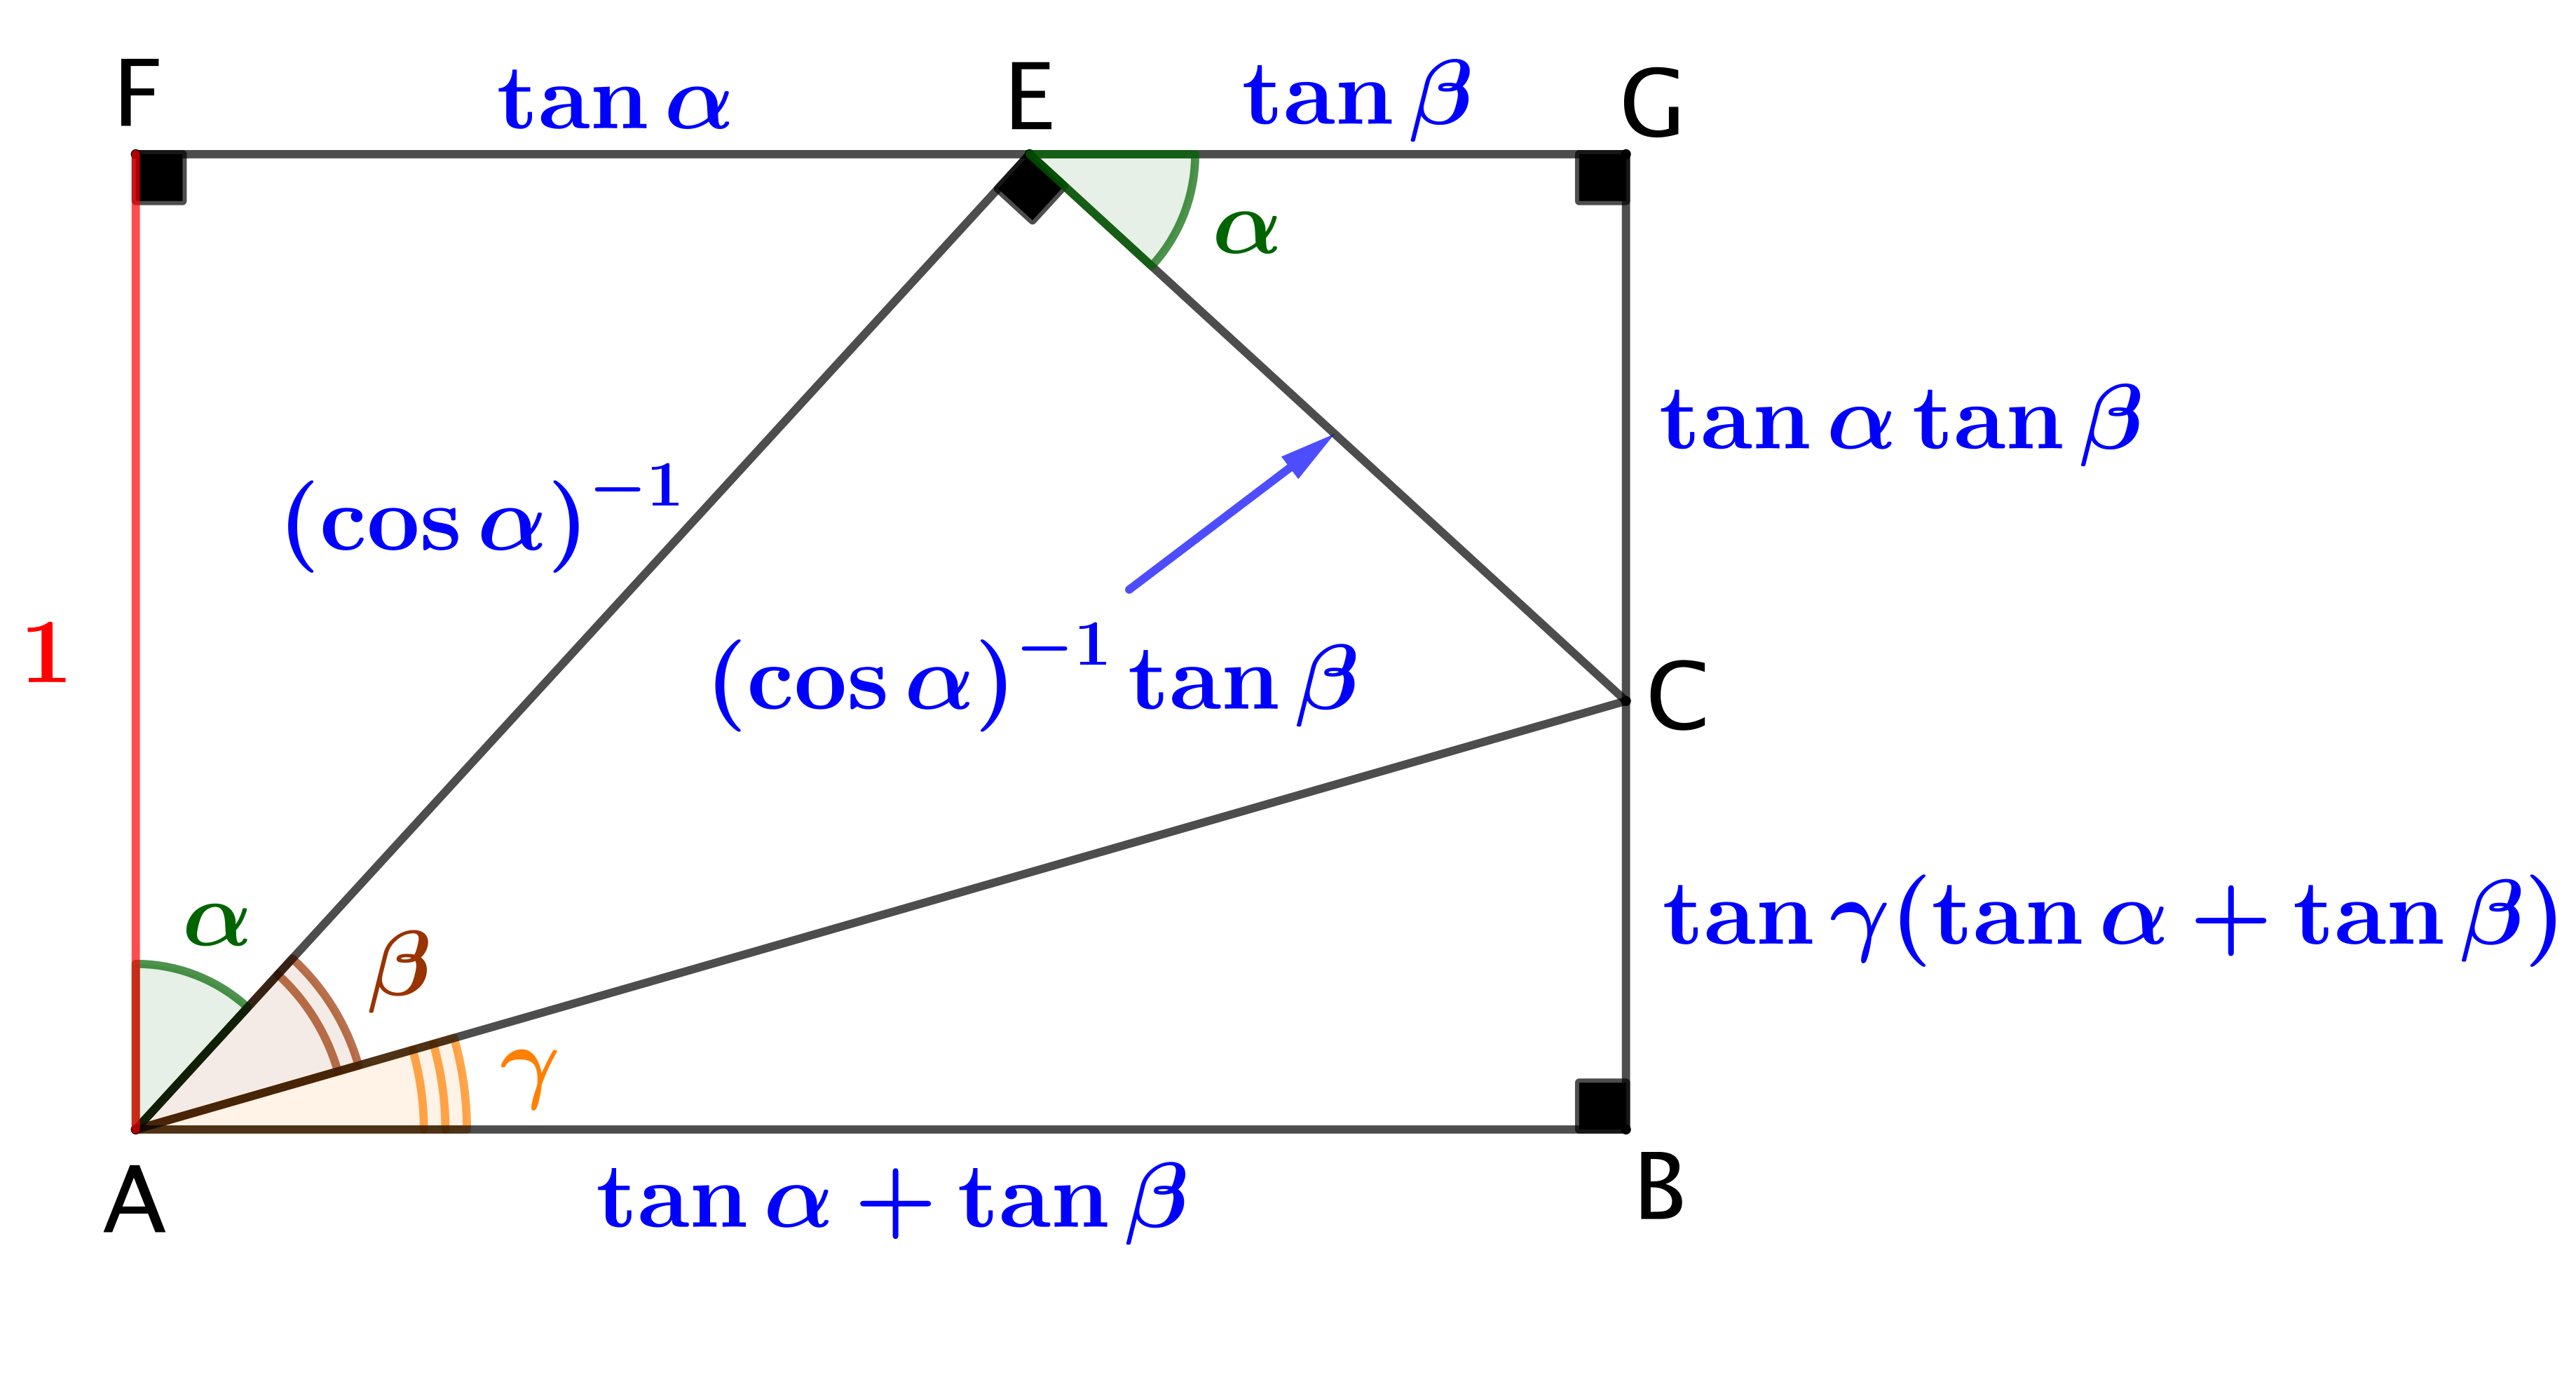
\includegraphics[scale=.75]{sum-tan-prod.png}
    \end{center}
    
%    \newpage
    
    Voici comment arriver à une généralisation pour
    $(\alpha ; \beta ; \gamma) \in \big( \CC - \frac{\pi}{2} \ZZ \big)^3$.
    %
    \begin{itemize}
    	\item Pour $(\alpha ; \beta) \in \big( \RRsp \big)^2$ tel que $0 < \alpha + \beta < \frac{\pi}{2}$,
		en posant $\gamma = \frac{\pi}{2} - \alpha - \beta$,
		le dessin donne
        %
        $
            \tan \alpha \tan \beta
            + \tan \beta  \tan \big( \frac{\pi}{2} - \alpha - \beta \big)
            + \tan \big( \frac{\pi}{2} - \alpha - \beta \big) \tan \alpha
            - 1
            = 0
        $.
        

    	\item En multipliant l'égalité précédente par 
		$\cos \alpha \cos \beta \cos \big( \frac{\pi}{2} - \alpha - \beta \big)$,
		nous obtenons la nullité sur $\intervalO{0}{\frac{\pi}{4}}^2$ d'une fonction $f(\alpha ; \beta)$ séparablement analytique.


    	\item Comme $\intervalO{0}{\frac{\pi}{4}}^2$ est discriminant, le \reffact{sep-isolated-zero} donne la nullité de $f(\alpha ; \beta)$ sur $\CC^2$.


    	\item Si
		$(\alpha ; \beta) \in \big( \CC - \frac{\pi}{2} \ZZ \big)^2$
		et
		$\frac{\pi}{2} - \alpha - \beta \in \CC - \frac{\pi}{2} \ZZ$,
		en divisant par
		$\cos \alpha \cos \beta \cos \big( \frac{\pi}{2} - \alpha - \beta \big)$,
		et
		en posant $\gamma = \frac{\pi}{2} - \alpha - \beta$,
		nous obtenons la généralisation à $(\alpha ; \beta ; \gamma) \in \big( \CC - \frac{\pi}{2} \ZZ \big)^3$ de l'implication initiale.
    \end{itemize}
\end{example}
